\chapter{Background}
\label{chapter1}

This project aims to improve the efficiency of real-time rendering of 3D fractals. This chapter will focus on background theory for fractals, signed distance functions and sphere tracing.

\section{2D Fractals - The Mandelbrot Set}

\begin{figure} \label{figure:mandelbrot-2d-full}
	\centering
	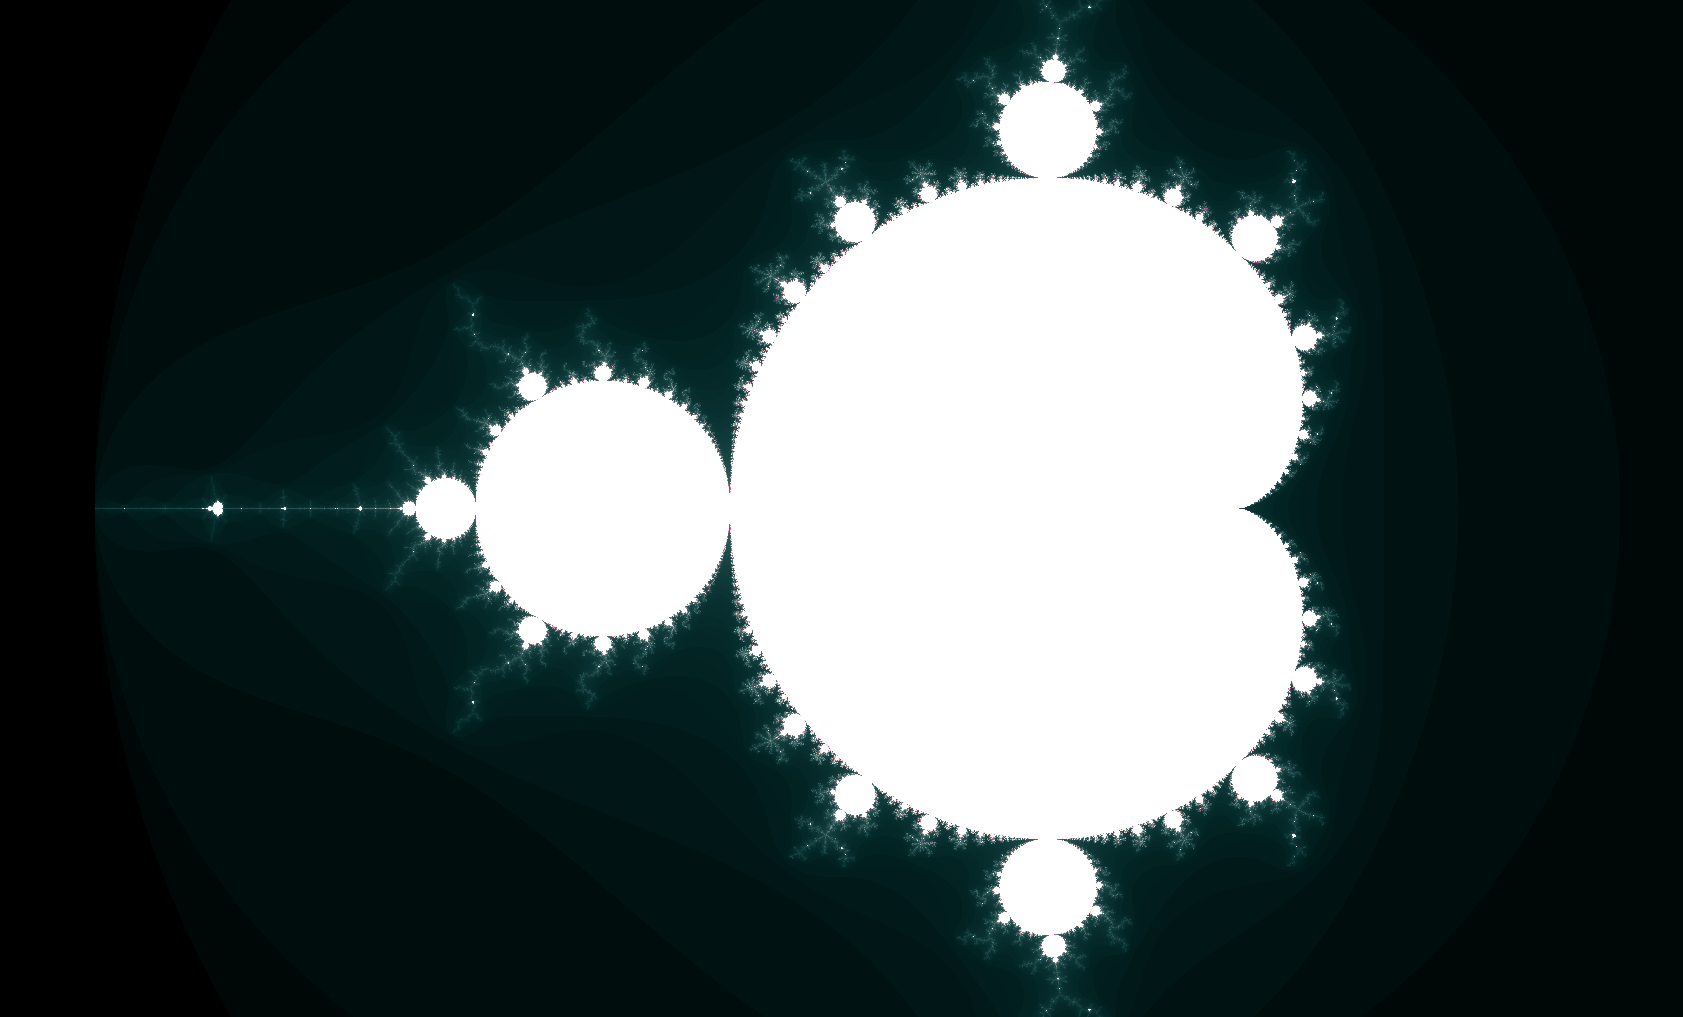
\includegraphics[width=0.75\linewidth]{Images/Mandelbrot-2D-Full.png}
	\caption{The Mandelbrot set. The white points in the centre are inside the set.}
\end{figure}

The Mandelbrot set is the set of two-dimensional points that satisfy a certain constraint on the following complex quadratic equation:

\begin{equation} \label{equation:mandelbrot-2d}
	Z = {Z^2} + C
\end{equation}

where Z and C are complex numbers. The constraint on the points is that their orbit must be bounded. The value of Z is initialized to 0 and equation \ref{equation:mandelbrot-2d} is iterated over, each new value of Z being placed back in to the equation in the next iteration. If the length of the point Z does not exceed a threshold, then the point (represented by C) is in the Mandelbrot set \cite{devaney1999mandelbrot}.

Figure \ref{figure:mandelbrot-2d-full} shows a generated Mandelbrot set. In this case, the real part of the point C is represented by the x-axis, and the imaginary part by the y-axis. Equation \ref{equation:mandelbrot-2d} is iterated over a maximum of five hundred times, and the threshold value is two. The pixels are coloured according to how many iterations are achieved before the length of Z exceeds the threshold.

The image presented in figure \ref{figure:mandelbrot-2d-full} ranges from negative one to one on the y-axis (and is proportional in the x-axis), but the Mandelbrot set has infinite detail, so if one decreases the range of the axes, new patterns will emerge. Figure \ref{figure:mandelbrot-2d-zoom} shows two zoomed-in views of the edge of the original shape. New patterns can be seen, as well as repeated ones, and even new instances of the original shape.

\begin{figure} \label{figure:mandelbrot-2d-zoom}
	\centering
	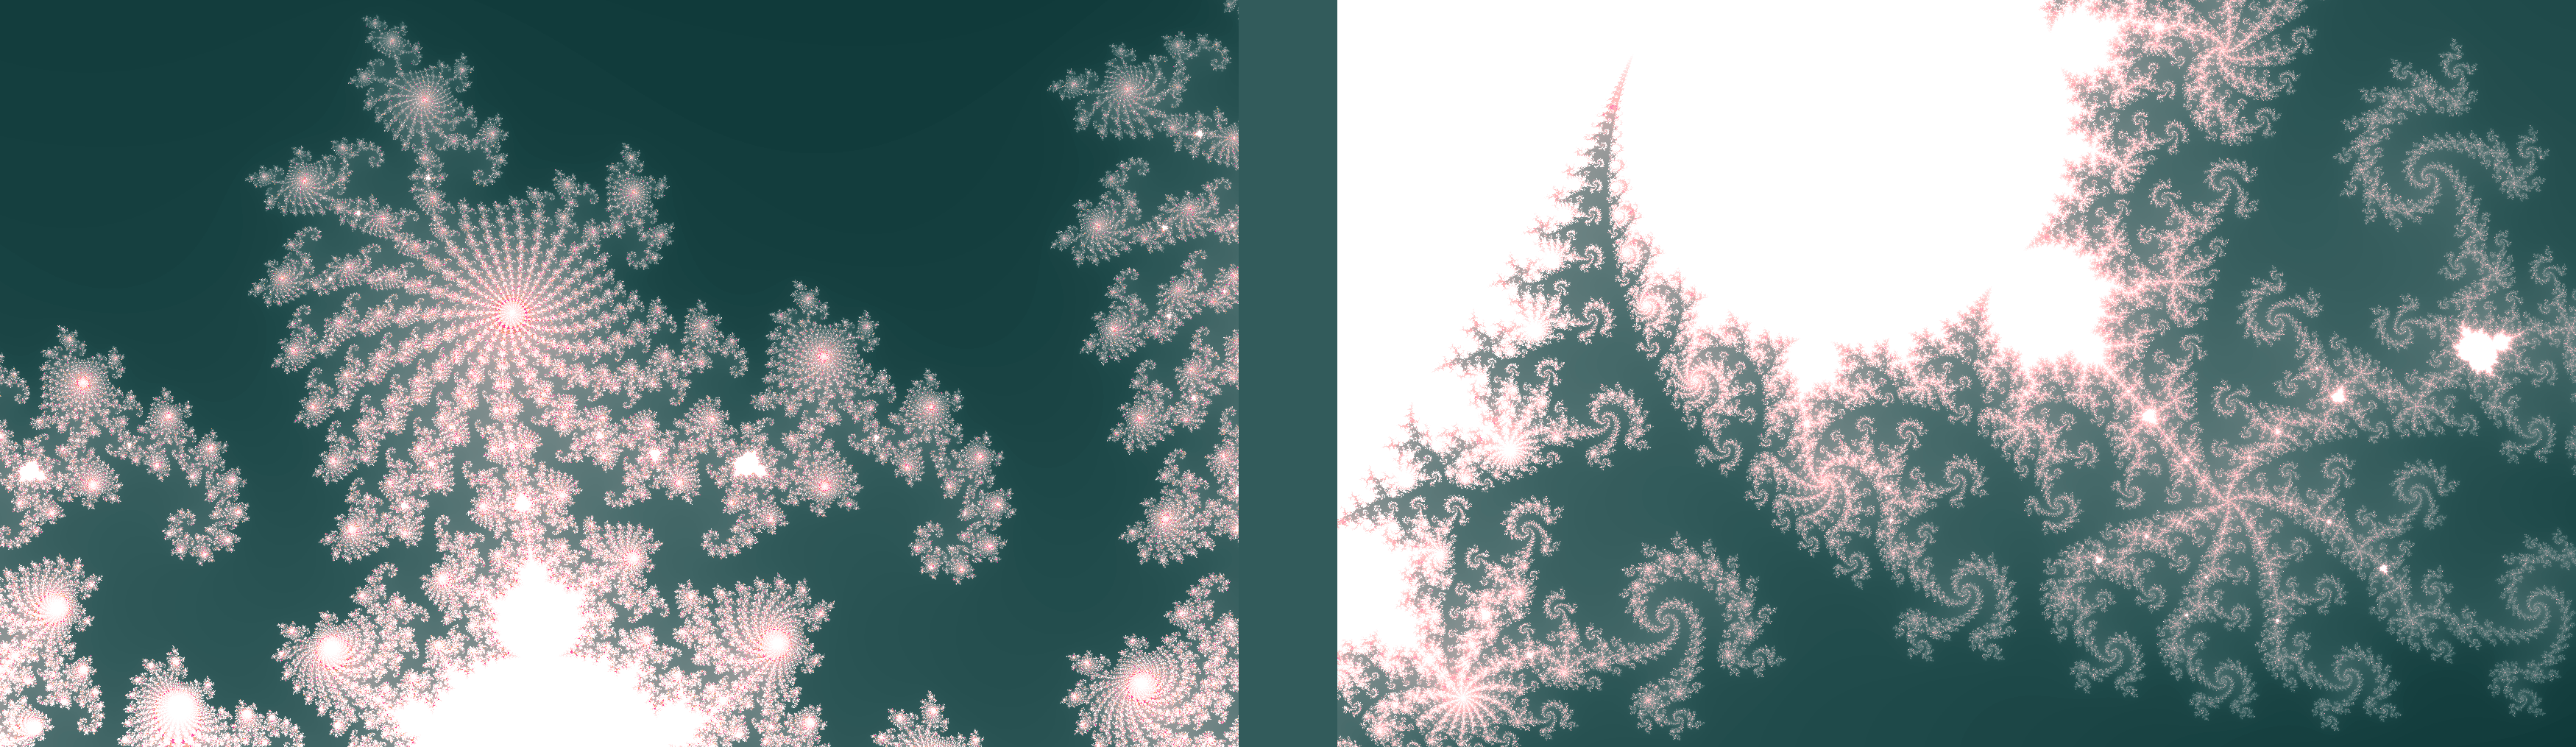
\includegraphics[width=\linewidth]{Images/Mandelbrot-2D-Zoom.png}
	\caption{The Mandelbrot set}
\end{figure}

Papers:
\begin{itemize}
	\item Similarity between the Mandelbrot set and Julia sets \cite{lei1990similarity}.
	\item Evolutionary exploration of the mandelbrot set \cite{ashlock2006evolutionary}.
	\item The Mandelbrot set, the Farey tree, and the Fibonacci sequence \cite{devaney1999mandelbrot}.
\end{itemize}

\section{3D Fractals - The Mandelbulb}

Papers:
\begin{itemize}
	\item The mandelbulb: first ‘true’3D image of famous fractal \cite{aron2009mandelbulb}.
\end{itemize}

\cite{aron2009mandelbulb}

- A few ways to represent mandelbrot in 3D.

- 1. Slices of 2D mandelbrot.

- 2. Quaternion mandelbrot with fourth dimension = 0.

- 3. Informal extension to 3D with polar coordinates.

- Explain each. I will be going with option 3.

\section{Signed Distance Functions and Sphere Tracing}

Papers:
\begin{itemize}
	\item Ray Tracing Gems II \cite{marrs2021ray}.
\end{itemize}

- Signed distance function is an estimate of how close the point is to the surface of the fractal.

-  If it's negative, the point is inside the surface.

- Demonstrate derivation from Mandelbulb equation.

- Distance estimators can be used for raymarching - known as sphere tracing.

- Diagram of sphere tracing.

\section{Signed Distance Fields}

Papers:
\begin{itemize}
	\item Signed distance fields: A natural representation for both mapping and planning \cite{oleynikova2016signed}.
\end{itemize}

- Stored values from signed distance function, stored as 2D texture or 3D grid.

- Saves having to recompute SDF all the time.

- Fractal scenes with high view distance could benefit from some pre-calculated values to give them a head start - show room of pillars and remark on frame rate (no SDF).

- Remark on memory costs.

- Briefly talk about storage methods - octrees.